
%%%%%%%%%%%%%%%%%%%%%%%%%%%%%%%%%%%%%%%%%
% задача оптимального выбора группы объектов и алгоритм для её решения
%%%%%%%%%%%%%%%%%%%%%%%%%%%%%%%%%%%%%%%%%
\subsection{Проблема выбора объектов}

Деятельность любых экономических субъектов, будь то организации, предприятия, госкорпорации, научные институты, домашние хозяйства или частные лица, направлена на получение выгоды за счёт затраты определённых ресурсов. Как правило, выгоду нужно максимизировать или хотя бы ограничить снизу, а ресурсы ограничены сверху. 

Значительная часть ресурсов выделяется на инвестиции, т.\,е. покупку, развитие или создание неких объектов: промышленных и научных приборов, ценных бумаг, объектов недвижимости и т.\,д. А значит, встаёт проблема оптимального выбора группы объектов, которые будут приобретены, из некого множества $O$ объектов, доступных для выбора. Слово <<группа>> в названии настоящей работы и применительно к объектам инвестиций не подразумевает  математическое понятие группы; с точки зрения математики имеется в виду подмножество $d \subset O$. За проведение выбора отвечает лицо, принимающее решение.

В каждой ситуации та или иная стратегия и процедура выбора объектов может считаться оптимальной. Не все они интересны с математической точки зрения. Например, выбор можно произвести волевым образом: лицо, принимающее решение, из своих внутренних соображений самостоятельно делает выбор. Он может стать тривиальным, если объекты достаточно простые (с точки зрения оценки выгоды от их приобретения) и находятся в той предметной области, где лицо, принимающее решение, достаточно компетентно. Но если объекты сложные или не покрываются одной конкретной предметной областью, а находятся в самых разных предметных областях, то лицо, принимающее решение, скорее всего, уже по этой причине не будет достаточно компетентно для того, чтобы сделать оптимальный выбор. Тогда привлекается эксперт или коллектив экспертов.
% к этому абзацу нужны ссылки на другие примеры стратегий выбора в литературе (Миша?)

Возможны различные сценарии работы экспертов, из которых мы в настоящей работе рассмотрим следующий: для каждого объекта экспертам предлагается выставить оценку его <<качества>> $x \in X$, где $X$ --- числовое множество. Эксперт способен сделать это в силу своего опыта и глубоких знаний предметной области, даже если истинное значение <<качества>> объекта невозможно вычислить, по крайней мере, до инвестирования. Субъективность суждения эксперта не подразумевает запрета опираться в том числе и на объективную информацию: факты об исследуемых объектах, факты о предметной области в целом, факты о прошлом опыте удачного и неудачного выбора объектов. Но в математической модели мы не учитываем такую информацию и считаем, что эксперт извлекает оценку непосредственно из своего сознания. Неизвестность $x$ моделируется нечётким элементом $\tilde x$, для которого восстанавливается  распределение возможности $p_{\tilde x}(\cdot): X \rightarrow \zo$, см. раздел <<Экспертные оценки и методы теории возможностей Ю.~П.~Пытьева>>. Таким образом, $p_{\tilde x}(\cdot)$ --- экспертная оценка $x$.    
% к этому абзацу нужны ссылки на другие примеры экспертных заданий в литературе
% убрал слово "лучших" (тавтология+ какие мы выбираем, ещё вопрос)

Обычно <<качество>> объекта, выраженное одним числом $x \in X$, --- недостаточно конкретное понятие для понимания экспертами того, что, собственно, надо оценивать. Поэтому заказчик экспертного опроса в качестве предварительного этапа работы с экспертами или до обращения к ним выявляет некоторые параметры оцениваемых объектов, часто называемые также <<критериями>> оценки. Хотя можно представить себе ситуацию, когда это не так, мы будем исходить из того, что каждый объект можно оценить по одним и тем же $m$ параметрам: $x_1 \in X_1, ..., x_m \in X_m$.  Поскольку заказчику важно не только то, какие параметры объектов оценивают эксперты, но и то, как эти параметры формируют итоговую оценку $x$, он разрабатывает формулу: $x = f(x_1, ..., x_m)$, где на функцию $f$ могут накладываться ограничения в зависимости от алгоритма, используемого для обработки оценок. Например, если все параметры имеют одинаковую важность, можно положить $x = \frac{1}{m}\sum_{j=1}^m{x_j}$.

%Экспертные оценки бывают разные по информативности и существуют разные математические теории для их моделирования  и анализа... 
% этой хрени достаточно во вводных разделах 

Итак, в настоящей работе используется следующая методика экспертного опроса:
\begin{center} \fbox{ 
\begin{minipage}{0.9 \textwidth}
 Экспертам предлагается выставить оценку в виде отображения $X \rightarrow \zo$ для каждого параметра каждого объекта из множества $O$. Эти оценки моделируются и анализируются с помощью теории возможностей Ю.~П.~Пытьева, причём никакая информация, кроме самих экспертных оценок, не учитывается в модели. Делается вывод о том, приобретение какие объектов является наиболее выгодным для заказчика экспертного опроса и можно ли сделать такой выбор.
\end{minipage}
} \end{center}

Теперь поставим математическую задачу, выражающую суть изложенной проблемы, и опишем компьютерный алгоритм для нахождения её решения. Будем пока считать, что есть только один эксперт, или же есть экспертный коллектив, но он действует единодушно. Если каждый эксперт может действовать независимо и выдаёт свой собственный набор оценок, то перед использованием нижеизложенного алгоритма следует по каждому параметру каждого объекта рассчитать оценку, выражающую коллективное мнение экспертов. Как это можно сделать, описано в разделе <<Оценка, выражающая коллективное мнение группы экспертов>>.

\subsection{Постановка задачи на минимум}

Пусть имеется $n$ объектов, причём множество $O = \{1, ..., n\}$ есть множество их индексов, и для оценки <<качества>> объектов приглашён $1$ эксперт. Ему предложено оценить каждый объект по $m$ параметрам, истинные значения которых неизвестны. 

Пусть моделью параметров служат нечёткие элементы $\tilde x_{ij}$. Не ограничивая общности, будем считать, что все они принимают значения на одном и том же числовом множестве $X$, т.\,е. значения параметров имеют вид $x_{ij} \in X$ для параметра с номером $j \in \{1, ..., m\}$ объекта с номером $i \in \{1, ..., n\}$. Экспертом заданы функции распределения $\p_{ij}(\cdot): X \rightarrow \zo$ нечётких элементов $\tilde x_{ij}$. <<Качество>> $i$-го объекта $x_i \in X$ выражается через $x_{ij}$ с помощью заднной заказчиком экспертизы монотонной по каждому аргументу функции $f$:
\begin{equation}
  \label{e:function_f}
  x_i = f(x_{i1}, ..., x_{im}),\,i = 1, ..., n.
\end{equation}

Введём нечёткий вектор $\theta = (\tilde x_{11}, ..., \tilde x_{nm})$, принимающий значения на множестве $\Om = X^{n \times m}$, которое состоит из всевозможных векторов $t = (x_{11}, ..., x_{nm})$. %T состоит из векторов t, а Омега из событий вида {тета=t}, но у них одинаковая размерность.
Будем считать, что его компоненты попарно независимы, что предполагает попарную независимость как параметров каждого объекта, так и самих объектов. Тогда $\theta$ имеет распределение: 
\begin{equation} 
	\label{e:p_theta_def}
	\p_{\theta}\big((x_{11}, ..., x_{nm})\big) = \inf_{i, j}\,\p_{ij}(x_{ij}),
\end{equation}
и порождает пространство с возможностью $\OAP$, где мера возможности любого события $A \subset \Om$ выражается через $\p_{\theta}(\cdot)$: 
\begin{equation} 
	\label{e:P_theta_def}
	\P(A) = \underset{t \in A} \sup\;\p_{\theta}(t). 
\end{equation}

Пространство $\OAP$ можно интерпретировать как модель нечёткого эксперимента $\Exp$. Эксперимент  заключается в измерении истинных значений параметров всей совокупности объектов. В реальности он никогда не проводится, т.\,к. его проведение означало бы приобретение сразу всех объектов. Эксперт восстанавливает возможностную модель эксперимента $\Exp$. Наблюдаемые величины и априорная информация отсутствуют.

Требуется выбрать $k$ из $n$ объектов, $1 \leq k < n$, т.\,е. подмножество $d \subset O$ размера $\abs{d} = k$. Множество всех таких подмножеств обозначим $D$. Допустим на минуту, что известны истинные значения $x_1, ..., x_n$, которые получаются с помощью (\ref{e:function_f}) из реализации $t = (x_{11}, ..., x_{nm})$ нечёткого вектора $\theta$. Тогда оптимальным выбором будет подмножество строго наиболее <<качественных>> объектов $\delta_t$:
\begin{equation}
    \label{e:delta_def}
    \delta_{t} \define= \{i_1, ..., i_k\}: \forall i \in \delta,\; \forall i' \in O \setminus \delta: x_i > x_{i'}. 
\end{equation}
Подмножество $\delta_{t}$ будем называть верным решением задачи о выборе объектов при $\theta = t$. Оно существует не всегда. Действительно, если расположить $x_1, ..., x_n$ в порядке невозрастания, из определения (\ref{e:delta_def}) следует:
\begin{equation*}
   % \label{e:right_order_strict}
    \delta_{t} = \{i_1, ..., i_k\}: x_{i_1} \geq ... \geq x_{i_k} > x_{i_{k+1}} \geq ... \geq x_{i_n},   
\end{equation*}
то есть между $x_{i_k}$ и $x_{i_{k+1}}$ должен стоять знак строгого неравенства. Но в общем случае цепочка выглядит так:
\begin{equation}
    \label{e:right_order}
    x_{i_1} \geq ... \geq x_{i_k} \geq x_{i_{k+1}} \geq ... \geq x_{i_n},   
\end{equation}
при некоторых $t$, $k$ между $x_{i_k}$ и $x_{i_{k+1}}$ может стоять знак равенства, и тогда не существует подмножества $\delta_t \subset O$ размера $\abs{\delta} = k$, которое  удовлетворяло бы (\ref{e:delta_def}). Это значит, что при таких $t$ и $k$ нельзя выбрать ровно $k$ лидеров. 

Пусть $\Eps(d)$ --- событие (все те ситуации $t$), при котором $d \in D$ не является верным решением:
\begin{equation*}
 % \label{e:Eps_d_def}
  \Eps(d) \define= \{t: \exists i \in d,\; \exists i' \in O \setminus d: x_i \leq x_{i'}\}.
\end{equation*}
Здесь  $x_i$ и $x_{i'}$, как и раньше, получены из координат $t$ с помощью (\ref{e:function_f}), и использовано отрицание (\ref{e:delta_def}). Поставим задачу оптимального выбора объектов как задачу минимизации возможности события $\Eps(d)$:
\begin{equation}
  \label{e:zadacha}
  \P(\Eps(d)) \sim \underset{d \in D} \min.
\end{equation}

\subsection{Формальное решение $d_*$ задачи на минимум  через определение $\P(\Eps_l)$}

Пусть $\Eps_l$ --- событие, при котором объект с индексом $l \in O$ не попал в число лидеров, т.\,e. найдётся хотя бы $k$ объектов, не совпадающих с $l$-м, <<качество>> которых не меньше $x_l$. Теперь, при выбранном решении $d$, событие $\Eps(d)$ возникает тогда и только тогда, когда один из объектов $l \in d$ не попал в число лидеров.\footnote{Для произвольных $d \in D$, $l \in d$ возникшее событие $\Eps_l$ означает, что найдётся хотя бы $k$ объектов, не совпадающих с $l$-м, <<качество>> которых не меньше $x_l$. Тогда выполняется условие появления $\Eps(d)$: $\exists i' \notin d: x_l \leq x_{i'}$, потому что $\abs{\{i: i \in d, i \neq l\}} = k-1$. Обратно, если возникло $\Eps(d)$, то для $l = \arg\min \{x_i:\,i \in d\}$ не только $k-1$ оставшихся объектов из $d$, но и как минимум один объект $i' \notin d$  будет не менее <<качественным>>, чем объект $l$, а значит, таких объектов --- как минимум $k$.} Поэтому: 
\begin{equation*}
  \Eps(d) = \bigcup_{l \in d} \Eps_l,
\end{equation*}
и с учётом правила суммирования возможностей можно записать:
\begin{equation}
  \label{e:razbienie}
  \P(\Eps(d)) = \sup_{l \in d} \P(\Eps_l).
\end{equation}

Если посчитать для каждого объекта $l \in O$ возможность не войти в число лидеров $\P(\Eps_l)$ и отсортировать объекты по неубыванию этих величин:
\begin{equation}
  \label{e:left_order}
  \P(\Eps_{l_1}) \leq ... \leq \P(\Eps_{l_k}) \leq \P(\Eps_{l_{k+1}}) \leq ... \leq \P(\Eps_{l_n}), 
\end{equation}
то $d_* = \{l_1, ...,  l_k\}$ будет решением задачи (\ref{e:zadacha}). Действительно, положив в (\ref{e:razbienie}) $d = d_*$, получим $\P(\Eps(d)) = \P(\Eps_{l_k}) = P_*$, а заменив какой-нибудь элемент  решения на $l_r$, $r > k$, получим $\P(\Eps(d)) = \P(\Eps_{l_r}) \geq P_*$. 

\subsection{Алгоритм нахождения $\P(\Eps_l)$}
 Итак, задачу (\ref{e:zadacha}) мы свели к задаче нахождения $\P(\Eps_l)$, $l \in O$. В соответствии с (\ref{e:p_theta_def}), (\ref{e:P_theta_def}):
\begin{equation}
  \label{e:pl_main}
  \P(\Eps_l) = \sup_{(x_{11}, ..., x_{nm})\,\in\,\Eps_l} \, \inf_{i, j}\,\p_{ij}(x_{ij}). 
  % заданы какие-то конкретные параметров x_{ij}, и уже потом по ним берётся супремум, поэтому p_{ij}(x_{ij}) 
  % эксперт же задаёт p_{ij}(x) при всех значениях х, т.е. функции p_{ij}()
\end{equation}

Узким местом формулы (\ref{e:pl_main}) при вычислении <<в лоб>> является перебор векторов $t \in \Om$ для проверки на предмет включения в $\Eps_l$, поскольку $\abs{\Om} = \abs{X}^{n \times m}$. Но оказывается, для приближённого нахождения $\P(\Eps_l)$ с точностью $\epsilon = 2^{-N}$ полный перебор делать не нужно: достаточно перебрать всего $N-1$ векторов. Дело в том, что можно относительно просто проверить отношение $\P(\Eps_l) > p$ для любого заданного числа $p \in \zo$ в силу транзитивности операций сравнения действительных чисел, лежащих в основе <<работы>>  $\sup$ и $\inf$, и монотонности функции $f$ (\ref{e:function_f}) по всем аргументам. 

Будем искать $\P(\Eps_l)$ отдельно для каждого конкретного $l \in O$ методом дихотомии. В качестве начального приближения $p^{(0)}$ возьмём середину отрезка $[p^{min(0)}, p^{max(0)}] = \zo$, поскольку любая возможность лежит на этом отрезке. На $i$-ом шаге, $i = 0, ..., N$ проверяем утверждение $\P(\Eps_l) > p^{(i)}$, а затем:
\begin{gather*}
 \P(\Eps_l) > p^{(i)} \Rightarrow 
    \left[ 
      \begin{gathered} 
        p^{min(i+1)} = p^{(i)}, \hfill 
        \\ 
        p^{max(i+1)} = p^{max(i)}. \hfill 
        \\ 
      \end{gathered} 
    \right. \\ 
 \P(\Eps_l) \leq p^{(i)} \Rightarrow 
    \left[ 
      \begin{gathered} 
        p^{min(i+1)} = p^{min(i)}, \hfill 
        \\ 
        p^{max(i+1)} = p^{(i)}. \hfill 
        \\ 
      \end{gathered} 
    \right. \\
 p^{(i+1)} = \frac{1}{2}\big(p^{min(i+1)} + p^{max(i+1)}\big).  
\end{gather*}
Таким образом, каждый следующий отрезок поиска в два раза короче предыдущего. На заданной $N$-ой итерации: $\abs{p^{max(N)} - p^{min(N)}} < 2^{-N}$ и $\P(\Eps_l) \approx p^{(N)}$. %$\frac{1}{2}(p^{min(N)} + p^{max(N)})$. 

Трудности могли бы возникнуть в тех случаях, когда истинное значение $\P(\Eps_l)$ равно $0$ или $1$, поскольку эти числа имеют особый смысл в теории возможностей, а также когда для каких-либо $l_1 \neq l_2$ $\P(\Eps_{l_1}) = \P(\Eps_{l_2})$. Но, во-первых, при анализе совокупности результатов $p^{(N)}$ и $[p^{max(N)} - p^{min(N)}]$ для разных $l$ такие случаи часто хорошо видны. Во-вторых, существует подход, при котором можно получить не приближенное, а точное значение $\P(\Eps_l)$. Достаточно вместо непрерывного множества значений возможности $\zo$ взять конечный набор, например, $Y = \{0.0, 0.1, 0.2, ..., 1.0\}$. Легко заметить, что операции $\sup$ и $\inf$ не выводят за пределы этого <<дискретизированного>> множества значений, поэтому $\P(\Eps_l) \in Y$, если исходный материал --- экспертные оценки $\p_{ij}(\cdot): X \rightarrow Y$ (что в определённом смысле удобно и для экспертов). Тогда при $N = 5 \Rightarrow 2^{-N} < 0.05$ можно $p^{(N)}$ однозначно отнести к $\P(\Eps_l) \in Y$.

Пусть $p \in \zo$. Для проверки утверждения $\P(\Eps_l) > p$ выполним следующие действия: 
\begin{enumerate}
  \item 
  Для каждого $i \in \{1, ..., n\}$, $j \in \{1, ..., m\}$ найдём подмножество $X_{ij} \define= \{x \in X: p_{ij}(x) > p\} \subset X$. 
  \item 
  Предположим, что параметры объекта $l$ приняли минимальные значения <<качества>> среди $X_{lj}$, а параметры всех остальных объектов, наоборот, --- максимальные значения в <<своём>> множестве. А именно, определим $t^\text{edge} = \{x_{ij}^\text{edge}\}$ следующим образом:
  \begin{equation*}
    x_{ij}^\text{edge} =
    \begin{cases}
      \min X_{ij}, &\text{если $i = l$.}\\
      \max X_{ij}, &\text{если $i \neq l$.} 
    \end{cases}
  \end{equation*}
  \item
  Рассчитаем итоговое <<качество>> всех объектов $x_i^\text{edge} = f(x_{i1}^\text{edge}, ..., x_{im}^\text{edge})$ с учётом нашего предположения и проверим, попадает ли $l$-й объект в $k$ лидеров. Для этого количество $q$ объектов, не совпадающих с $l$-м, <<качество>> которых не меньше $x_l$, сравниваем с $k$:
 	\begin{itemize}
		\item если $q < k$, то $\P(\Eps_l) \leq p$.
		\item в противном случае, $\P(\Eps_l) > p$.
	\end{itemize} 
\end{enumerate}  

Действительно, поскольку в теории возможностей верно
\begin{equation*}
 % \label{e:transitive}
  \P(A) > a \Leftrightarrow \exists\;\omega \in A: \p(\omega) > a,
\end{equation*}
то в силу (\ref{e:pl_main}) утверждение $\P(\Eps_l) \leq p$ истинно, если и т.\,если у всех векторов $t \in \Eps_l$ хотя бы одна координата $x_{ij}$ такова, что $\p_{ij}(x_{ij}) \leq p$. А значит, противоположное утверждение $\P(\Eps_l) > p$ истинно, если и т.\,если найдётся хотя бы один вектор $t \in \Eps_l$, у которого все координаты $x_{ij} $ будут лежать в соответствующих подмножествах $X_{ij} = \{x \in X: p_{ij}(x) > p\}$. 

%Осталось выяснить, лежит ли он в $\Eps_l$.
Координаты вектора $t^\text{edge}$, полученного в пункте~2, есть $\{x_{ij}^\text{edge}\} \in X_{ij} \forall\,i, j$.  
Если $t^\text{edge} \in \Eps_l$, то в силу описанной выше эквивалентности делается вывод $\P(\Eps_l) > p$. Если же $t^\text{edge} \notin \Eps_l$, как ни старались мы туда его <<запихнуть>> выбором самых <<невыгодных>> значений параметров, то и никакой другой вектор $t$ с координатами $x_{ij} \in X_{ij}$ не лежит в $\Eps_l$ в силу монотонности функции $f$. Действительно, замена каких-либо координат $t^\text{edge}$ на более <<выгодные>> для $l$-го объекта не уменьшает $x_l^\text{edge} = f(x_{l1}^\text{edge}, ..., x_{lm}^\text{edge})$ и не увеличивает $x_i^\text{edge} = f(x_{i1}^\text{edge}, ..., x_{im}^\text{edge})$, $i \neq l$ в цепочке (\ref{e:right_order}).

Фактически, на множестве $\Om$ можно ввести отношение линейного псевдопорядока (см. раздел про методы теории упорядоченных множеств). Пусть $\Pi_l(\cdot): \Om \rightarrow \setN$ --- позиция $l$-го объекта в цепочке (\ref{e:right_order}), считая слева направо. Она монотонно зависит от $t \in \Om$ в силу монотонности $f$, причём $\Pi_l (t)$ --- целые числа с естественной упорядоченностью, которая и порождает упорядоченность векторов $t$ с точностью до того, что несколько различных $t$ могут соответствовать одному и тому же $\Pi_l(t)$. 

Событие $\Eps_l$ начинается с $t: \Pi_l(t) = k+1$, а событие $A = \{t = (x_{11}, ..., x_{nm}): x_{ij} \in X_{ij}\}$ либо пересекается, либо не пересекается с $\Eps_l$ (см.~рис.~\ref{ris:algo_sets}). Если $\Eps_l \not\intersects A$, то их можно разделить прямой $\{\Pi_l(t) = \Pi_l(t^\text{edge})\}$, которая обозначена пунктиром на рисунке.

\begin{figure}[h]
\center{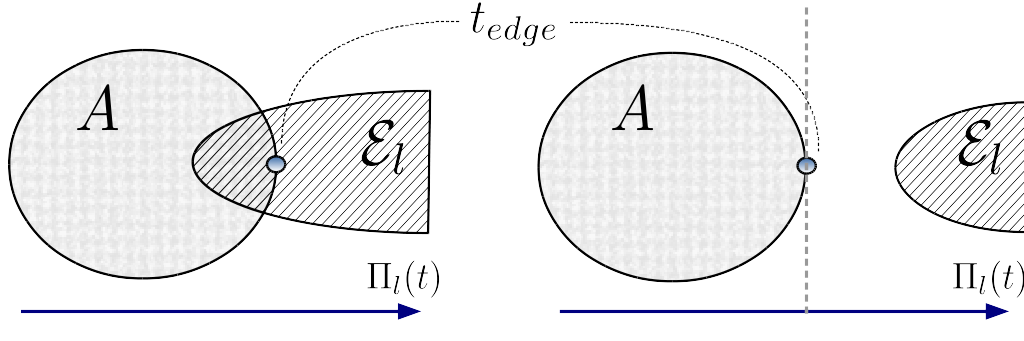
\includegraphics[width=0.85\linewidth]{./pic/algo_sets2}}
\caption{\small Иллюстрация взаимного расположения исследуемых событий и построенного вектора $t_{edge}$ в случае $\P(\Eps_l) > p$ (справа) и в случае $\P(\Eps_l) \leq p$ (слева) для заданного $p \in \zo$.}
\label{ris:algo_sets}
\end{figure}

\subsection{Анализ корректности решения $d_*$}
\subsubsection*{Замечание 1}

%Может возникнуть неоднозначность выбора $d_*$, связанная с наличием знаков равенства в цепочке (\ref{e:left_order}). 
Пусть в цепочке (\ref{e:left_order}) $P_* = \P(\Eps_{l_k}) = ... = \P(\Eps_{l_q}) < \P(\Eps_{l_{q+1}})$, $q \geq k$. По построению минимум (\ref{e:zadacha}) достигается на любом решении $d' \subset \Delta \define= \{l_1, ..., l_q\}$, $\abs{d'} = k$, и такое $d'$ сводится к $d_*$ простой заменой индексов. Если $q > k$, следует считать, что решение задачи оптимального выбора объектов не единственное, и сообщить об этом заказчику экспертного опроса. ЛПР может или отказаться от выбора вовсе, например, потребовав дополнительную экспертизу, или выбрать любые $k$ объектов из $\Delta$, или даже отказаться от исходного требования задачи и вместо $k$ выбрать $r$ объектов из $\Delta$, где $k \leq r \leq q$.

\subsubsection*{Замечание 2}
Пусть $E_0 = \{t: \nexists \delta(t)\}$. Это событие возникает, когда найдётся хотя бы $n-k+1$ объектов, для каждого из которых найдётся $k$ объектов не меньшей <<значимости>>:
\begin{equation*}
 E_0 = (\Eps_1 \cap ... \cap \Eps_{n-k+1}) \bigcup (\Eps_2 \cap ... \cap \Eps_{n-k+2}) \bigcup ... \bigcup (\Eps_{k-1} \cap ... \cap \Eps_{n}).
 % надо было бы объедиение по всем возможным наборам, но всё гораздо проще!
\end{equation*}
Событие $E_0$ --- более узкое, чем $\Eps_l$, где требуется $k$ объектов не меньшей <<значимости>> только для объекта $l$:
\begin{equation*}
 E_0 \subset \Eps_l \Rightarrow \Eps_l = E_0 \cup E_l,\;l \in O,
\end{equation*}
где $E_0$ состоит из векторов $t: \nexists \delta(t)$, которые войдут во все $\Eps_l$, а 
$E_l$ --- оставшаяся часть $\Eps_l$. По правилу сложения возможностей:
\begin{equation*}
 \P(\Eps_l) = \sup\{\P(E_0), \P(E_l)\}.
\end{equation*}
%Постоянное первое слагаемое зависит, прежде всего, от выбора $f$ (\ref{e:function_f}). Если оно больше, чем минимум второго слагаемого, для некоторых $l$, возможности таких $\Eps_l$ будут равны, а это может быть плохо для однозначности решения задачи (\ref{e:zadacha}). Поэтому в спорной ситуации, когда в цепочке (\ref{e:left_order}) много равенств, имеет смысл посмотреть на возможность $\P(E_0)$. Если она окажется равна многим $\P(\Eps_l)$, требуется выбрать другую функцию $f$. Если же нет, то спорная ситуация возникла только из-за экспертных $\p_{ij}$.